\scalebox{1} % Change this value to rescale the drawing.
{
\begin{pspicture}(0,-3.2514062)(9.6,3.2514062)
\rput(4.8,-0.33640626){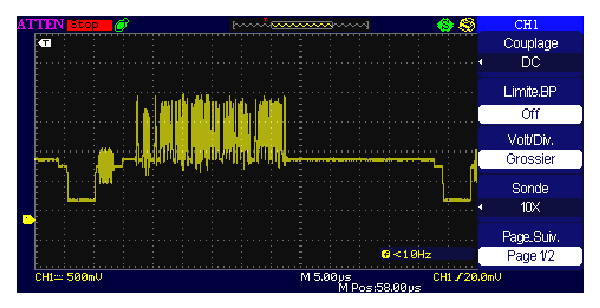
\includegraphics{images/1ligne.eps}}
\psframe[linewidth=0.05,linecolor=blue,dimen=outer](1.86,0.28359374)(0.2,-1.3364062)
\psframe[linewidth=0.05,linecolor=blue,dimen=outer](7.76,0.22359376)(6.78,-1.2964063)
\psframe[linewidth=0.05,linecolor=red,dimen=outer](6.72,0.76359373)(1.92,-1.3564062)
\usefont{T1}{ppl}{m}{n}
\rput(5.0892186,-3.0264063){Synchronisation de ligne}
\usefont{T1}{ppl}{m}{n}
\rput(5.1634374,3.0335937){Luminance pour une ligne}
\psline[linewidth=0.05cm,linecolor=red,arrowsize=0.153cm 2.0,arrowlength=1.4,arrowinset=0.4]{->}(3.64,2.8235939)(3.7,0.7835938)
\psline[linewidth=0.05cm,linecolor=blue,arrowsize=0.173cm 2.0,arrowlength=1.4,arrowinset=0.4]{->}(2.84,-2.8764062)(1.76,-1.3364062)
\psline[linewidth=0.05cm,linecolor=blue,arrowsize=0.153cm 2.0,arrowlength=1.4,arrowinset=0.4]{->}(6.8,-2.7964063)(7.02,-1.2964063)
\end{pspicture} 
}